\documentclass[14pt]{extbook}
\usepackage{multicol, enumerate, enumitem, hyperref, color, soul, setspace, parskip, fancyhdr} %General Packages
\usepackage{amssymb, amsthm, amsmath, latexsym, units, mathtools} %Math Packages
\everymath{\displaystyle} %All math in Display Style
% Packages with additional options
\usepackage[headsep=0.5cm,headheight=12pt, left=1 in,right= 1 in,top= 1 in,bottom= 1 in]{geometry}
\usepackage[usenames,dvipsnames]{xcolor}
\usepackage{dashrule}  % Package to use the command below to create lines between items
\newcommand{\litem}[1]{\item#1\hspace*{-1cm}\rule{\textwidth}{0.4pt}}
\pagestyle{fancy}
\lhead{Makeup Progress Quiz 2}
\chead{}
\rhead{Version A}
\lfoot{5763-3522}
\cfoot{}
\rfoot{Spring 2021}
\begin{document}

\begin{enumerate}
\litem{
Solve the rational equation below. Then, choose the interval(s) that the solution(s) belongs to.\[ \frac{-3}{-4x -6} + 6 = \frac{-9}{12x + 18} \]\begin{enumerate}[label=\Alph*.]
\item \( x_1 \in [-2.75, -0.75] \text{ and } x_2 \in [-2.25,-0.25] \)
\item \( \text{All solutions lead to invalid or complex values in the equation.} \)
\item \( x \in [0.25,3.25] \)
\item \( x \in [-1.75,0.25] \)
\item \( x_1 \in [-2.75, -0.75] \text{ and } x_2 \in [0.25,2.25] \)

\end{enumerate} }
\litem{
Determine the domain of the function below.\[ f(x) = \frac{4}{20x^{2} -35 x + 15} \]\begin{enumerate}[label=\Alph*.]
\item \( \text{All Real numbers except } x = a, \text{ where } a \in [11.91, 12.78] \)
\item \( \text{All Real numbers.} \)
\item \( \text{All Real numbers except } x = a \text{ and } x = b, \text{ where } a \in [0.31, 0.96] \text{ and } b \in [0.94, 1.52] \)
\item \( \text{All Real numbers except } x = a, \text{ where } a \in [0.31, 0.96] \)
\item \( \text{All Real numbers except } x = a \text{ and } x = b, \text{ where } a \in [11.91, 12.78] \text{ and } b \in [24.72, 25.13] \)

\end{enumerate} }
\litem{
Choose the equation of the function graphed below.
\begin{center}
    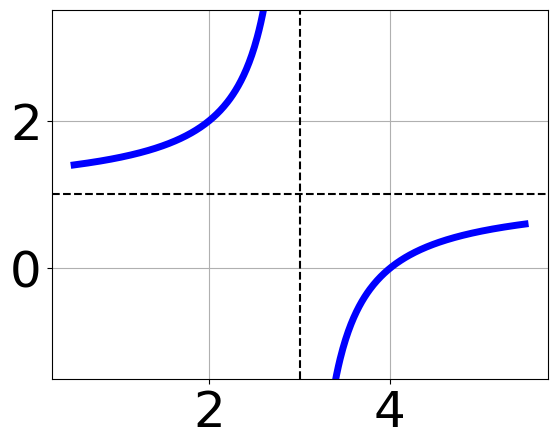
\includegraphics[width=0.5\textwidth]{../Figures/rationalGraphToEquationCopyA.png}
\end{center}
\begin{enumerate}[label=\Alph*.]
\item \( f(x) = \frac{1}{(x + 3)^2} + 1 \)
\item \( f(x) = \frac{-1}{x - 3} + 1 \)
\item \( f(x) = \frac{-1}{(x - 3)^2} + 1 \)
\item \( f(x) = \frac{1}{x + 3} + 1 \)
\item \( \text{None of the above} \)

\end{enumerate} }
\litem{
Choose the equation of the function graphed below.
\begin{center}
    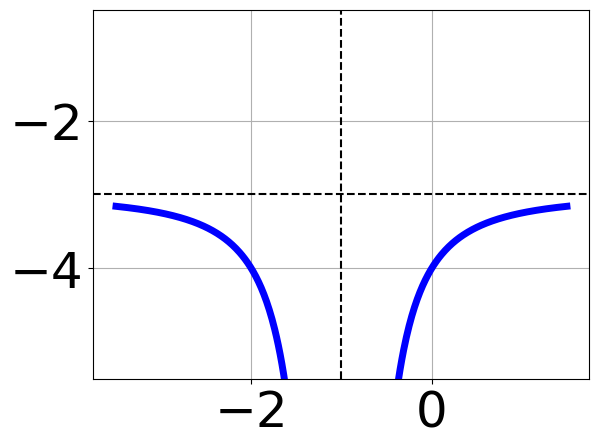
\includegraphics[width=0.5\textwidth]{../Figures/rationalGraphToEquationA.png}
\end{center}
\begin{enumerate}[label=\Alph*.]
\item \( f(x) = \frac{1}{(x - 1)^2} - 3 \)
\item \( f(x) = \frac{-1}{(x + 1)^2} - 3 \)
\item \( f(x) = \frac{1}{x - 1} - 3 \)
\item \( f(x) = \frac{-1}{x + 1} - 3 \)
\item \( \text{None of the above} \)

\end{enumerate} }
\litem{
Solve the rational equation below. Then, choose the interval(s) that the solution(s) belongs to.\[ \frac{7x}{-6x + 6} + \frac{-3x^{2}}{36x^{2} -78 x + 42} = \frac{5}{-6x + 7} \]\begin{enumerate}[label=\Alph*.]
\item \( x_1 \in [0.55, 0.62] \text{ and } x_2 \in [0.69,1.07] \)
\item \( x \in [1.16,1.18] \)
\item \( x_1 \in [0.55, 0.62] \text{ and } x_2 \in [1.07,1.48] \)
\item \( x \in [1.17,1.34] \)
\item \( \text{All solutions lead to invalid or complex values in the equation.} \)

\end{enumerate} }
\litem{
Solve the rational equation below. Then, choose the interval(s) that the solution(s) belongs to.\[ \frac{-9}{-6x -2} + 6 = \frac{-2}{-54x -18} \]\begin{enumerate}[label=\Alph*.]
\item \( x_1 \in [-1.4, -0.1] \text{ and } x_2 \in [-0.9,-0.3] \)
\item \( x \in [-1.58,1.42] \)
\item \( x \in [-0.2,1.3] \)
\item \( x_1 \in [-1.4, -0.1] \text{ and } x_2 \in [-0.5,0.9] \)
\item \( \text{All solutions lead to invalid or complex values in the equation.} \)

\end{enumerate} }
\litem{
Determine the domain of the function below.\[ f(x) = \frac{4}{25x^{2} +45 x + 20} \]\begin{enumerate}[label=\Alph*.]
\item \( \text{All Real numbers except } x = a \text{ and } x = b, \text{ where } a \in [-25.34, -24.97] \text{ and } b \in [-20.13, -19.86] \)
\item \( \text{All Real numbers except } x = a, \text{ where } a \in [-25.34, -24.97] \)
\item \( \text{All Real numbers except } x = a \text{ and } x = b, \text{ where } a \in [-1.15, -0.85] \text{ and } b \in [-0.87, -0.58] \)
\item \( \text{All Real numbers except } x = a, \text{ where } a \in [-1.15, -0.85] \)
\item \( \text{All Real numbers.} \)

\end{enumerate} }
\litem{
Choose the graph of the equation below.\[ f(x) = \frac{1}{x - 3} + 1 \]\begin{enumerate}[label=\Alph*.]
\begin{multicols}{2}\item 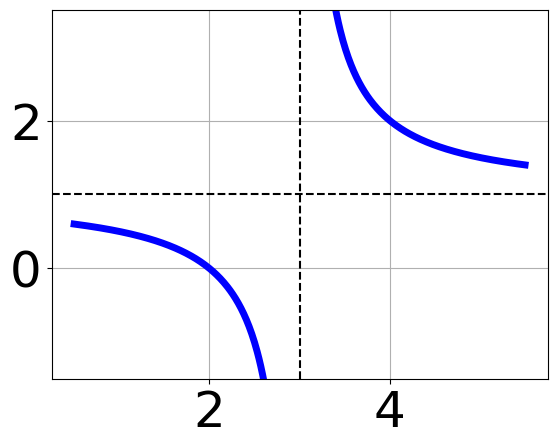
\includegraphics[width = 0.3\textwidth]{../Figures/rationalEquationToGraphCopyAA.png}\item 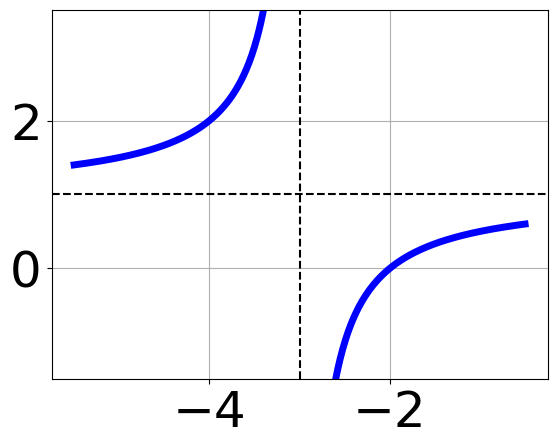
\includegraphics[width = 0.3\textwidth]{../Figures/rationalEquationToGraphCopyBA.png}\item 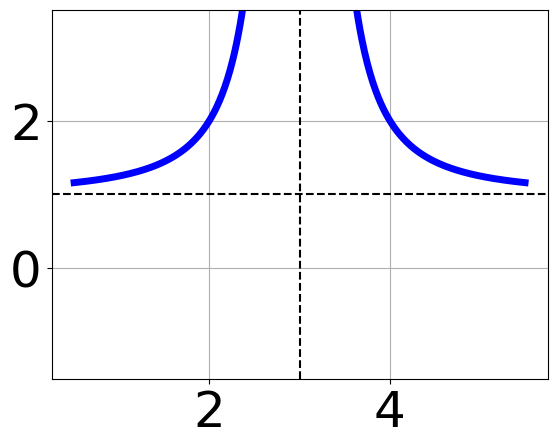
\includegraphics[width = 0.3\textwidth]{../Figures/rationalEquationToGraphCopyCA.png}\item 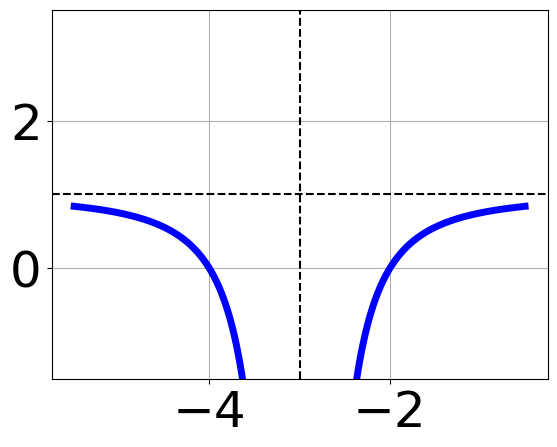
\includegraphics[width = 0.3\textwidth]{../Figures/rationalEquationToGraphCopyDA.png}\end{multicols}\item None of the above.
\end{enumerate} }
\litem{
Choose the graph of the equation below.\[ f(x) = \frac{-1}{x + 3} - 3 \]\begin{enumerate}[label=\Alph*.]
\begin{multicols}{2}\item 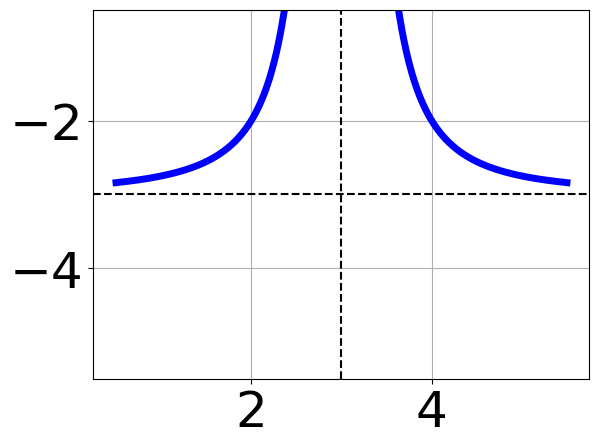
\includegraphics[width = 0.3\textwidth]{../Figures/rationalEquationToGraphAA.png}\item 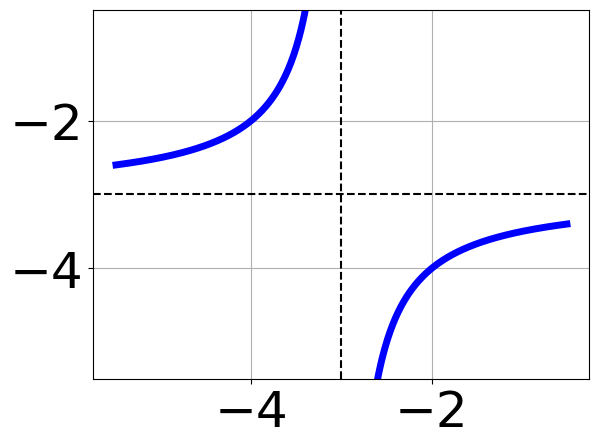
\includegraphics[width = 0.3\textwidth]{../Figures/rationalEquationToGraphBA.png}\item 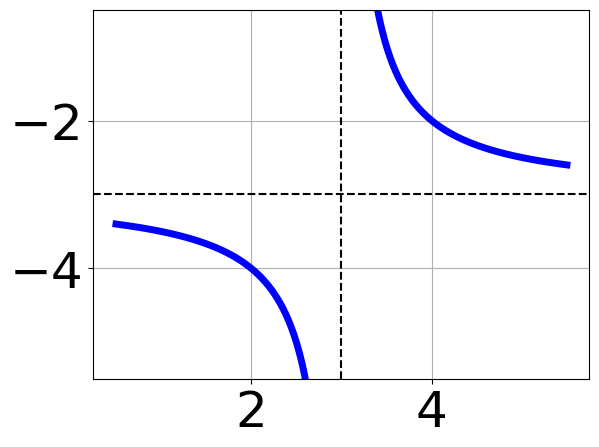
\includegraphics[width = 0.3\textwidth]{../Figures/rationalEquationToGraphCA.png}\item 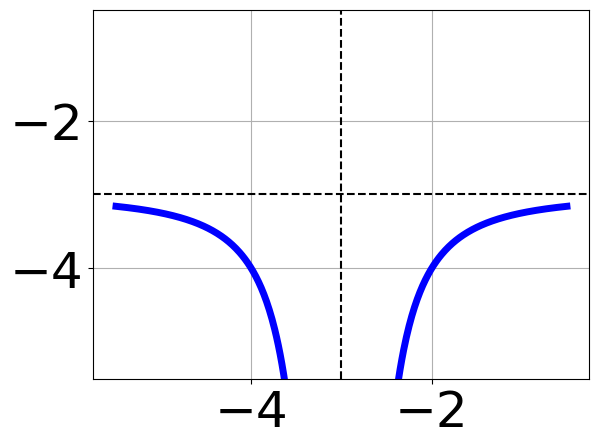
\includegraphics[width = 0.3\textwidth]{../Figures/rationalEquationToGraphDA.png}\end{multicols}\item None of the above.
\end{enumerate} }
\litem{
Solve the rational equation below. Then, choose the interval(s) that the solution(s) belongs to.\[ \frac{-3x}{-5x + 2} + \frac{-3x^{2}}{30x^{2} -27 x + 6} = \frac{-3}{-6x + 3} \]\begin{enumerate}[label=\Alph*.]
\item \( x \in [1.22,1.51] \)
\item \( x_1 \in [0.25, 0.37] \text{ and } x_2 \in [1.15,2.13] \)
\item \( x_1 \in [0.25, 0.37] \text{ and } x_2 \in [-1.09,0.72] \)
\item \( \text{All solutions lead to invalid or complex values in the equation.} \)
\item \( x \in [0.37,0.71] \)

\end{enumerate} }
\end{enumerate}

\end{document}